\documentclass[a4paper,10pt]{article}
\usepackage[utf8]{inputenc}
\usepackage{url}
\usepackage{enumerate}
\usepackage{verbatim}
\usepackage{graphicx}
\usepackage{changepage}% http://ctan.org/pkg/changepage
\usepackage{lipsum}% http://ctan.org/pkg/lipsum
\graphicspath{ {images/} }

%paragraph indentation
\setlength{\parindent}{4em} 

%paragraph spacing
\setlength{\parskip}{1em}

%Line spacing
% \renewcommand{\baselinestretch}{1.5}


\title{ \textbf{Study and Implementation of SDS}}

\author{ Supervisor - Prof. S C Gupta \\
Aashish Goyal (2012CS10202) \\
Devansh Dalal (2012CS10224)  }

\begin{document}

\maketitle

\abstract{This study aims to understand the relevance of software defined storage systems(SDS), which is the current state of the art in storage solutions. The study shall look at the shortcomings of older distributed storage solutions, the essential components of sds and how it addresses the shortcomings. Then it dives in to give an overview of the architecture of an open source solution -- Ceph. Finally it concludes by documenting our efforts to set up a virtual cluster using ceph. }    

\section{Introduction}
    SDS may be defined as a data storage method in which management and functioning of the data is abstracted from the actual physical storage and is controlled by software. The aim is create a system that can handle petabytes of data,  simplify the complexity associated with managing such a system, provide fault tolerance and self healing capabilities. We shall first look at older storage distributions and understand their limitations
    
\subsection{Traditional Storage Solutions}
    The most common storage solutions in this sphere are based on SAN or NAS. A storage area network (SAN) is a dedicated network that provides access to consolidated, block level data storage on which a file system can be mounted. Network-attached storage (NAS) is a file-level computer data storage server connected to a computer network providing data access to a heterogeneous group of clients --  a specialized computer built from the ground up for storing and serving files connected over the network. However both systems are plagued by scalability. To scale NAS to petabytes involves dealing with a lot of complexity and SAN are already complicated enough when used along with file-system.
    
    Moreover the functionality of legacy file systems such as appending, amending files, permissions etc. are not a good fit to today's use case. Most of the data that is currently being generated is unstructured and immutable .These features then only add to complexity, greater overhead and lot of meta-data management.Further the directory based structure of file-system which despite being extremely intuitive and useful also adds up to the complexity of locating the file in the files-ystem and complicates the REST API to access data in the cloud. RAID, the de-facto scheme for data protection also fails to scale. The scheme works well in small drives but as the data size increases the time to recover also increases. Long down-times are not acceptable by today's standards and hence alternatives such as replication or erasure coding need to be adopted.
    
\subsection{Object Storage}
    This is a storage architecture which manages data as objects rather than file systems which manage data as files in a hierarchy. The objects include the data, some associated meta-data and a uid (unique identifier) to search and access them. In case of updates to the data the entire object is replaced. Although this may seem as expensive and lacking in features at first, it turns out that the simplicity offered by such an organization of data makes it very easy to scale and manage. Further current usage pattern on data involves vast amount of immutable data and hence this pattern is also a good fit here. The meta-data in this case is associated with the object (not the file-system) and hence does not pose a barrier to scalability. Object storage is one of the most sought after features in modern storage systems.
    
\subsection{Components of SDS}
Here we look at the essential components that storage system must possess to qualify as a software defined storage.    

\begin{enumerate}[1]

\item  \textbf{\texttt{Abstraction }}  The storage resources are virtualized and presented to the control plane where they can be configured as needed

\item  \textbf{\texttt{Commodity Hardware }} These should be able to use easily available commodity hardware for storage as well as network needs. This leads to much lower operation costs compared to traditional solutions.

\item  \textbf{\texttt{Automation}} Should provide automation to provide policy-based provisioning of storage. The user need not dive into the inner details of physical configuration of drives when needing space, say for some application.  

\item  \textbf{\texttt{Resource Pooling }} The storage resources are pooled into a single logical entity and managed centrally by the control plane. 

\item  \textbf{\texttt{Elasticity }} It should be possible to add/remove storage devices from the cluster and also change the allocation of space to the user on the fly.

\item  \textbf{\texttt{Management Simplicity }} It is imperative that the system is easy to manage so that the skill and labour needed for implementing SDS is less.
\end{enumerate}


Object Storage and SDS is already in use by several large companies such as Google, Facebook, DropBox and Amazon to a name a few. Whereas this serves to validate the importance of these technologies, the implementations of these systems is proprietary. So instead we look at the Ceph storage which is amongst the most popular open source distributed file system. Not only does it have the above features but also has several others and builds on ideas of the highly successful Hadoop file-system.

\section{Ceph}

    Ceph \cite{cephwiki} is an open source distributed and software defined storage system designed keeping in view the demands today's storage demands. It builds up on the ideas of other distributed storage systems such as the vastly popular Hadoop file system and aims to address several shortcomings in these. Some of the improvements include no single point of failure ( in hadoop one has single metadata server, which if goes down the system is unusable), POSIX compliant with extra primitives for HPC(high performance computing), improved lookup latencies owing to replacing allocation tables with a deterministic algorithm which allows clients to compute where the object needed is stored(CRUSH) etc. The interested reader may learn more about the same by reading the research publications available here \cite{cephpub}.

Ceph is a free software storage platform designed to present object, block, and file storage from a single distributed computer cluster. Ceph's main goals are to be completely distributed without a single point of failure, scalable to the exabyte level, and freely-available. The data is replicated, making it fault tolerant.\cite{andrew}

Ceph software runs on commodity hardware. The system is designed to be both self-healing and self-managing and strives to reduce both administrator and budget overhead.

\begin{figure}[!htb]
% \advance\leftskip-0cm
% \advance\rightskip-1cm
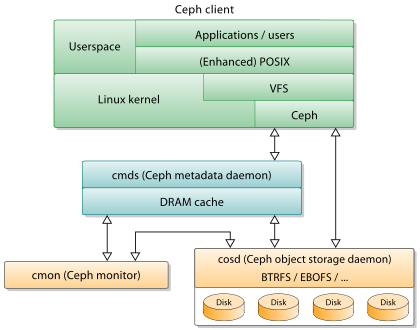
\includegraphics[width=12cm,height=10cm]{images/ceph1}
\caption[Long caption]{A high-level overview of the Ceph's internal organization}
\label{A high-level overview of the Ceph's internal organization}
\end{figure}

\subsection{Design}

Ceph employs four distinct kinds of daemons:
\begin{enumerate}[1]
\item  \textbf{\texttt{ceph-mon: }} A Ceph Monitor maintains a master copy of the cluster map. A cluster of Ceph monitors ensures high availability should a monitor daemon fail. Storage cluster clients retrieve a copy of the cluster map from the Ceph Monitor.

\item \textbf{\texttt{ceph-mds: }} Metadata servers (ceph-mds) that store the metadata of inodes and directories.

\item \textbf{\texttt{ceph-osd: }} Object storage devices (ceph-osd) that actually store the content of files. Ideally, OSDs store their data on a local btrfs filesystem to leverage its built-in copy-on-write capabilities, though other local filesystems can be used instead.

\item \textbf{\texttt{ceph-rgw :}} Representational state transfer gateway (ceph-rgw) that expose the object storage layer as an interface compatible with Amazon S3 or OpenStack Swift APIs.

\end{enumerate}


\begin{figure}[!htb]
\centering
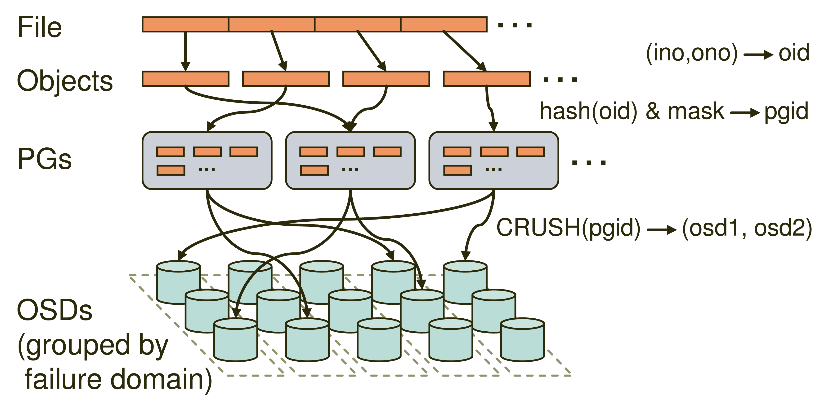
\includegraphics[width=9cm,height=5cm]{images/osd}
\caption[Long caption]{ ceph-storage overview }
\end{figure}

    All of these are fully distributed, and may run on the same set of servers. Clients directly interact with all of them. Ceph does striping of individual files across multiple nodes to achieve higher throughput, similarly to how RAID0 stripes partitions across multiple hard drives. Adaptive load balancing is supported whereby frequently accessed objects are replicated over more nodes.

\subsection{Architecture}

    Ceph uniquely delivers object, block, and file storage in one unified system. Ceph is highly reliable, easy to manage, and free. It has extraordinary scalability–thousands of clients accessing petabytes to exabytes of data. A Ceph Node leverages commodity hardware and intelligent daemons, and a Ceph Storage Cluster accommodates large numbers of nodes, which communicate with each other to replicate and redistribute data dynamically.

\begin{figure}[!htb]
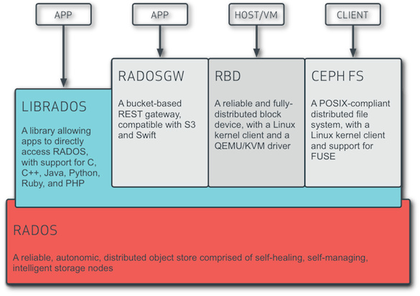
\includegraphics[width=12cm,height=10cm]{images/Ceph-view}
\caption[Long caption]{A high-level overview of Ceph's different ways for accessing stored data}
\end{figure}

\begin{adjustwidth}{1.5em}{0pt}
\subsubsection{\small{Storing Data}}
    In Ceph's storage cluster each object corresponds to a file in a file-system, which is stored on an Object Storage Device(OSD). Ceph OSD Daemons store all data as objects in a flat namespace and handle the read/write operations on the storage disks.
\end{adjustwidth}


\begin{adjustwidth}{1.5em}{0pt}
\subsubsection{\small{Scalability and Availability}}
    In traditional architectures, clients talk to a centralized component, which acts as a single point of entry to a complex subsystem. This imposes a limit to both performance and scalability, while introducing a single point of failure (i.e., if the centralized component goes down, the whole system goes down, too). Ceph eliminates the centralized gateway to enable clients to interact with Ceph OSD Daemons directly. Ceph OSD Daemons create object replicas on other Ceph Nodes to ensure data safety and high availability. Ceph also uses a cluster of monitors to ensure high availability. To eliminate centralization, Ceph uses the CRUSH algorithm .
\end{adjustwidth}

\begin{adjustwidth}{1.5em}{0pt}
\subsubsection{\small{High Availability Monitors}}
    Before Ceph Clients can read or write data, they must contact a Ceph Monitor to obtain the most recent copy of the cluster map. A Ceph Storage Cluster can operate with a single monitor; however, this introduces a single point of failure (i.e., if the monitor goes down, Ceph Clients cannot read or write data). So for added reliability and fault tolerance, Ceph supports a cluster of monitors. 
\end{adjustwidth}


\begin{adjustwidth}{1.5em}{0pt}
\subsubsection{\small{CRUSH Algorithm}}
    Ceph Clients and Ceph OSD Daemons both use the CRUSH\cite{crush} algorithm to efficiently compute information about object location, instead of having to depend on a central lookup table. CRUSH provides a better data management mechanism compared to older approaches, and enables massive scale by cleanly distributing the work to all the clients and OSD daemons in the cluster. CRUSH uses intelligent data replication to ensure resiliency, which is better suited to hyper-scale storage. 
\end{adjustwidth}


\begin{figure}[!htb]
\centering
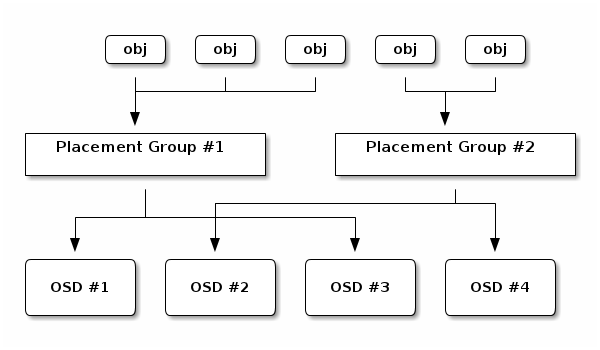
\includegraphics[width=10cm,height=7cm]{images/crush}
\caption[Long caption]{Assignment of osds to placement group is done using \emph{CRUSH} }
\end{figure}


\subsection{Comparison}
    Ceph has a number of features which make it very attractive for the massive growth in data in recent years (also referred to as big data). It has been designed for scalability, reliability, and performance. At the same time it assumes that failure of hardware is common, so it has been designed to adapt to these situations. Ceph breaks the file system into two pieces: (1) metadata, and (2) data. Separation of concerns allows ceph to implement an efficient and clean design for both parts.\cite{lwn}

    Ceph uses a dynamic distributed metadata server (MDS) that is not only clustered but also adapts to the changing workload. It will automatically distribute portions of the hierarchical directory tree to other MDS servers in the cluster to better load balance as the workload changes. In addition, if a MDS server is added, it will move portions of the metadata to that new box, again, improving the load distribution.
    
    Ceph's popularity is however nowhere close to that of the Hadoop file-system. Hadoop has only one metadata server and if it goes down entire system goes down. So it has only single point of failure and difficult to scale due to centralization of mds. Further object storage is not baked into the architecture of hadoop unlike ceph. Where hadoop wins out is the eco-system around it. Being widely popular it is already in use by several large organizations and has several additional components and layers on top of it. Numerous research papers around hadoop are available and even jobs are readily available. Despite being around for a long time ceph is yet to reach 1.0 and jobs are scarce. However having the solid foundation that it has the ceph may dominate the future.


\subsection{Implementation}
    Here we shall briefly describe our efforts to set up a virtual ceph cluster. The setup involved four virtual machines (minimum) running on two physical machines. The virtualization software used was virtual box and the operating system on the virtual machines was ubuntu 14.04. Note that the space available for each vm (especially those which are to be used as OSDs later) must be greater than 30GB. Initial attempts to use another lighter virtualization software namely lxc were not successful as lxc shares/uses the host operating systems kernel. To allow the storage to be used as a service we decided to use a bridged network in virtual box.


    The process of setting up the cluster is straightforward. Using the ceph-deploy tool ceph was installed on one of the nodes. The first node was called admin-node and used to subsequently administer the cluster. As host name resolution service was not accessible, the /etc/hosts file was edited to allow local resolution. The ceph cluster was then installed on each node using the ceph-deploy tool. Details of the installation and scripts to automate the process are available.
    
    After installing the ceph cluster a pool was created to serve as a block storage device. Over this (virtual) block device the ext3 file-system was mounted and then used as a file-system. By installing a ceph-client on any (compatible) device on the network it became possible to use this file-system as a resource. The next logical step would be to attempt to set-up a physical cluster comprising several nodes and test if it can be reliably used as a file-system for needs of the department and as a replacement to the expensive solution currently in place.

\medskip

\bibliographystyle{unsrt}%Used BibTeX style is unsrt
\bibliography{sample}

\end{document}
